\begin{figure}[t]
\centering
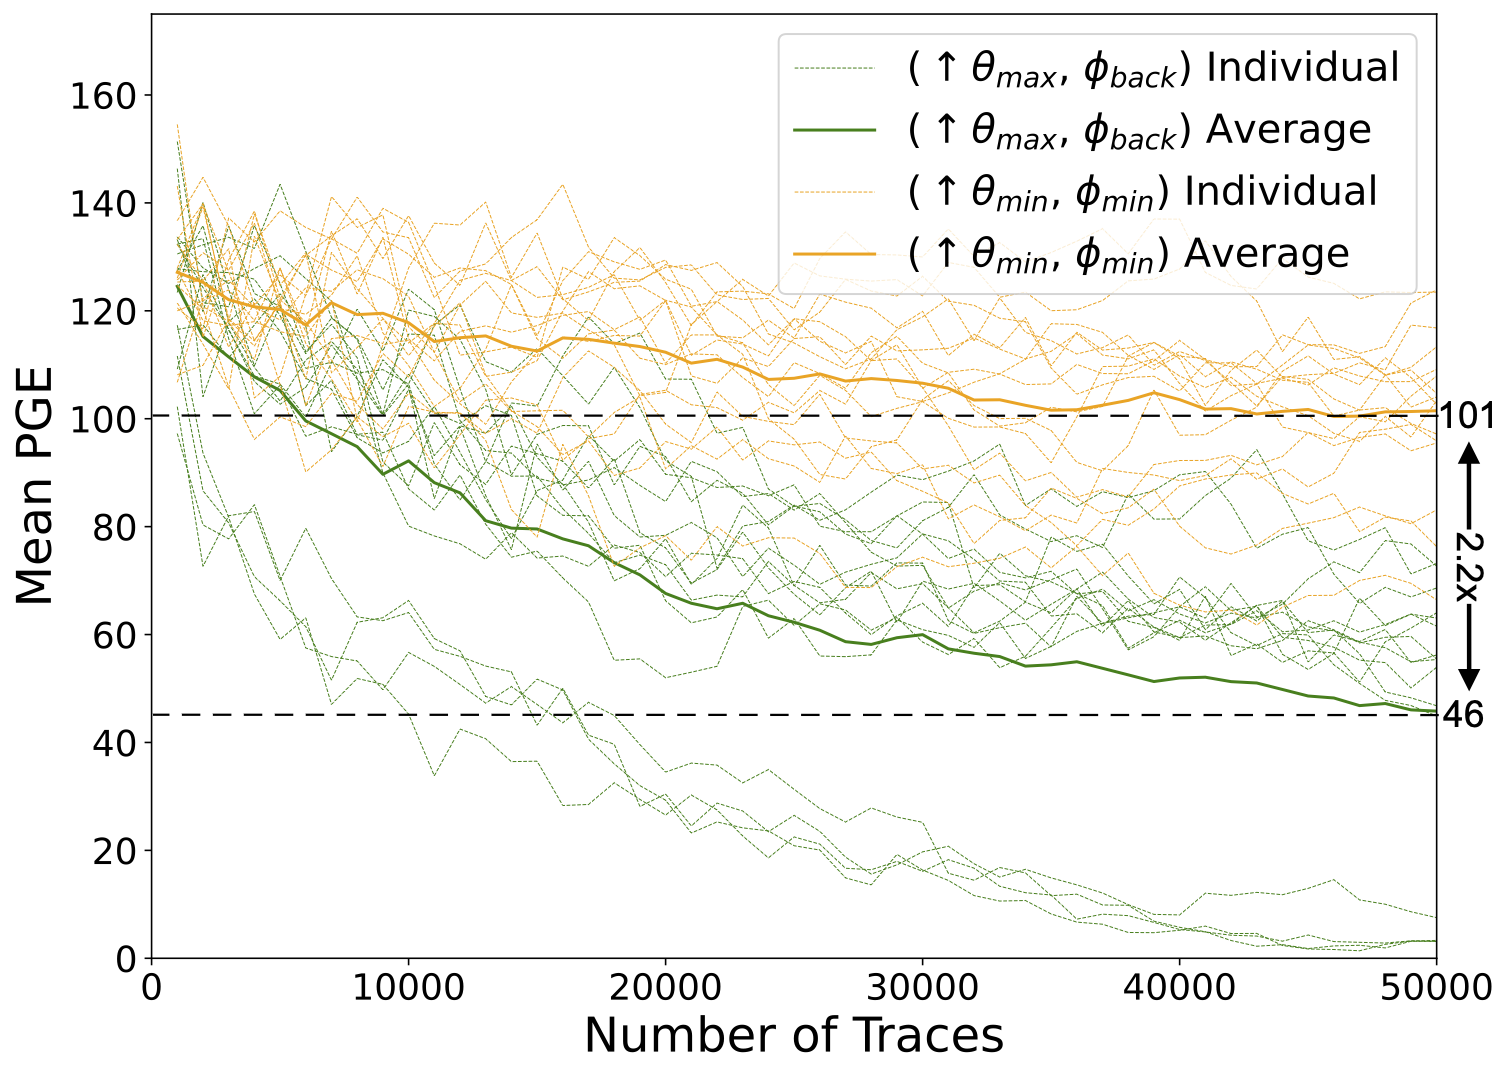
\includegraphics[width= 0.6\linewidth]{img/mean_pge_vs_traces.png}\\
\vspace{-10px}
\caption{Performance of a CPA attack for ($\uparrow\theta_{max}$, $\phi_{back}$) and ($\uparrow\theta_{min}$, $\phi_{min}$) tuning parameters. Lower average PGE indicates that the attack is performing better, as the correct subkey values are ranked as more likely after processing fewer traces. Our tuning method has a significant impact on key recovery, lowering PGE by 2.2$\times$ at 50,000 traces.}
\label{fig:mean-pge}
\vspace{-12px}
\end{figure}